In this section, the results obtained will be shown and compared. Each solution was tested on the proposed graphs in \ref{sec:graph} to verify their behavior in different contexts. 
The test has been executed on \textbf{Xeon PHI}, with $64$ cores and $4$ hardware thread per core. 

In the table (\ref{table:seq_times}) below, are included the sequential times used in the plots and to compute the speedup of the various solutions.
\begin{table}[htb!]
\centering
\begin{tabular}{|c|c|c|c|}
\hline
Sequential & 10K 0.02D & 10K 0.5D & 10K 0.8D \\ \hline
Time ($\mu sec$)          & 21964     & 162399   & 359583   \\ \hline
\end{tabular}
\caption{Time results of the sequential executions.}
\label{table:seq_times}
\end{table}
\FloatBarrier

The following plots show the performance trend of the proposed solutions, starting from the low dense graph. The tests of the dynamic scheduling version were performed with chunk size of $32$, $64$ and $128$. 

In this first graph, with density equal to $0.02$, all the four solution have the same behavior also for the performance drop around the $10$ workers. Moreover, the dynamic solution with chunk size of $128$ the knee point comes before due the smaller size of the frontiers.
\begin{figure}[htb!]
    \centering
    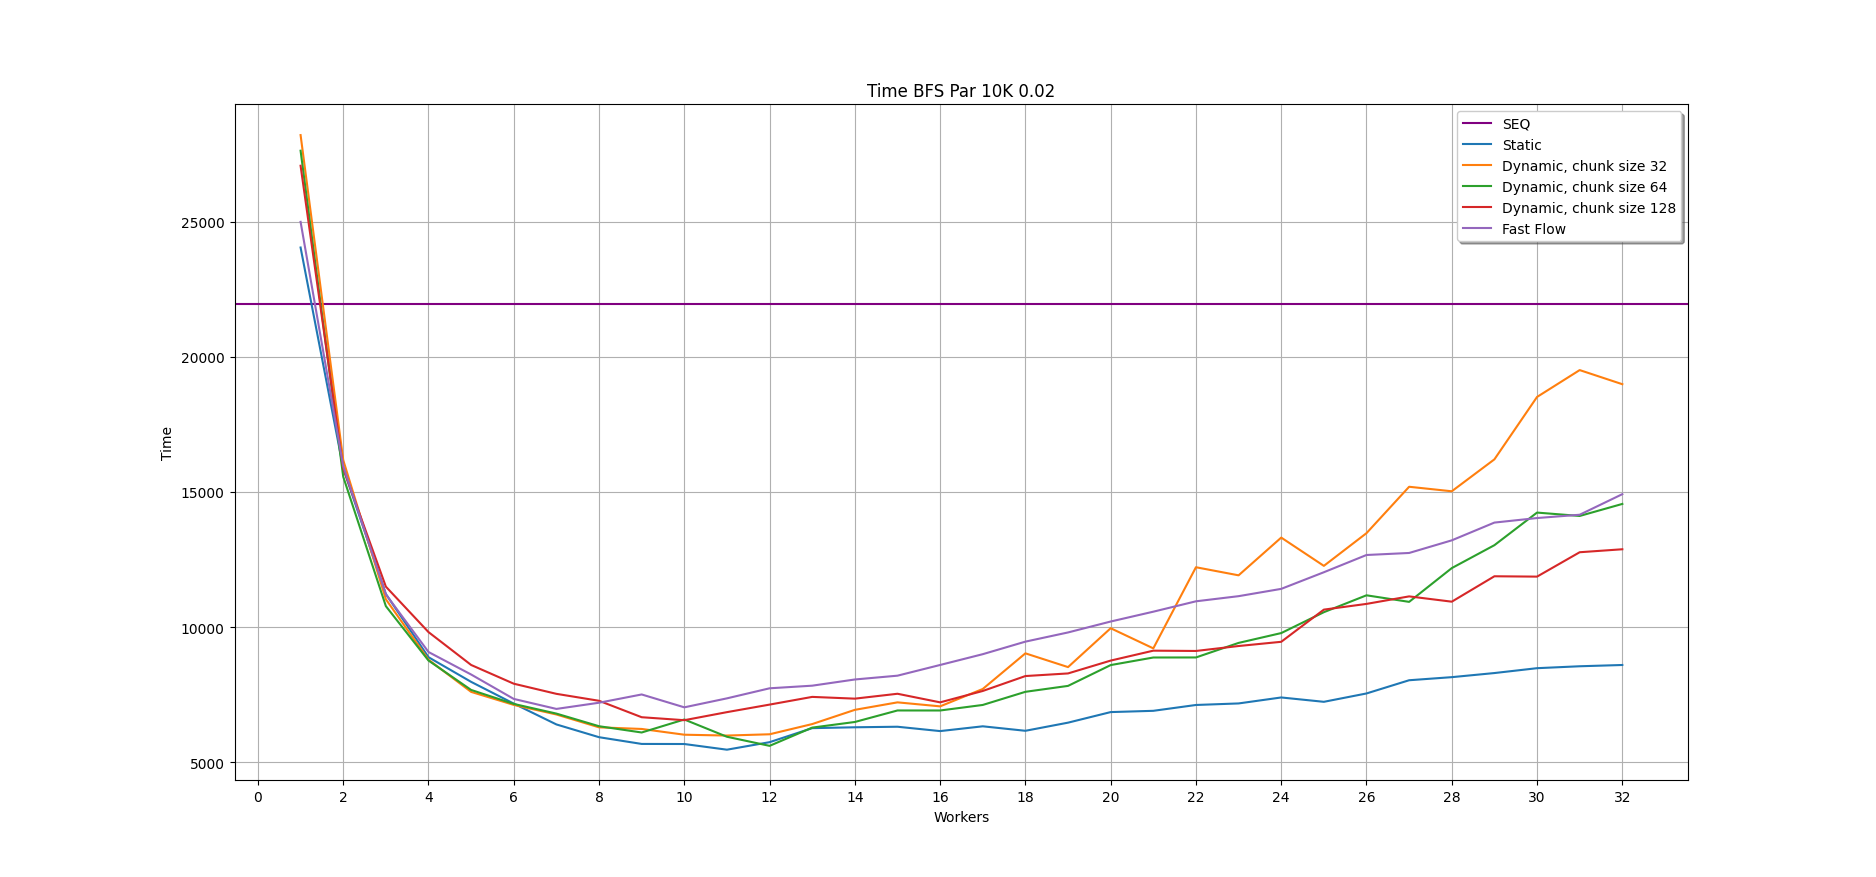
\includegraphics[width=0.75\textwidth]{Figures/plot_map_time_vs10K002.png}
    \caption{Time plot graph 0.02 density.}
    \label{fig:plot_time_10k_002}
\end{figure}
\FloatBarrier

\begin{figure}[htb!]
    \centering
    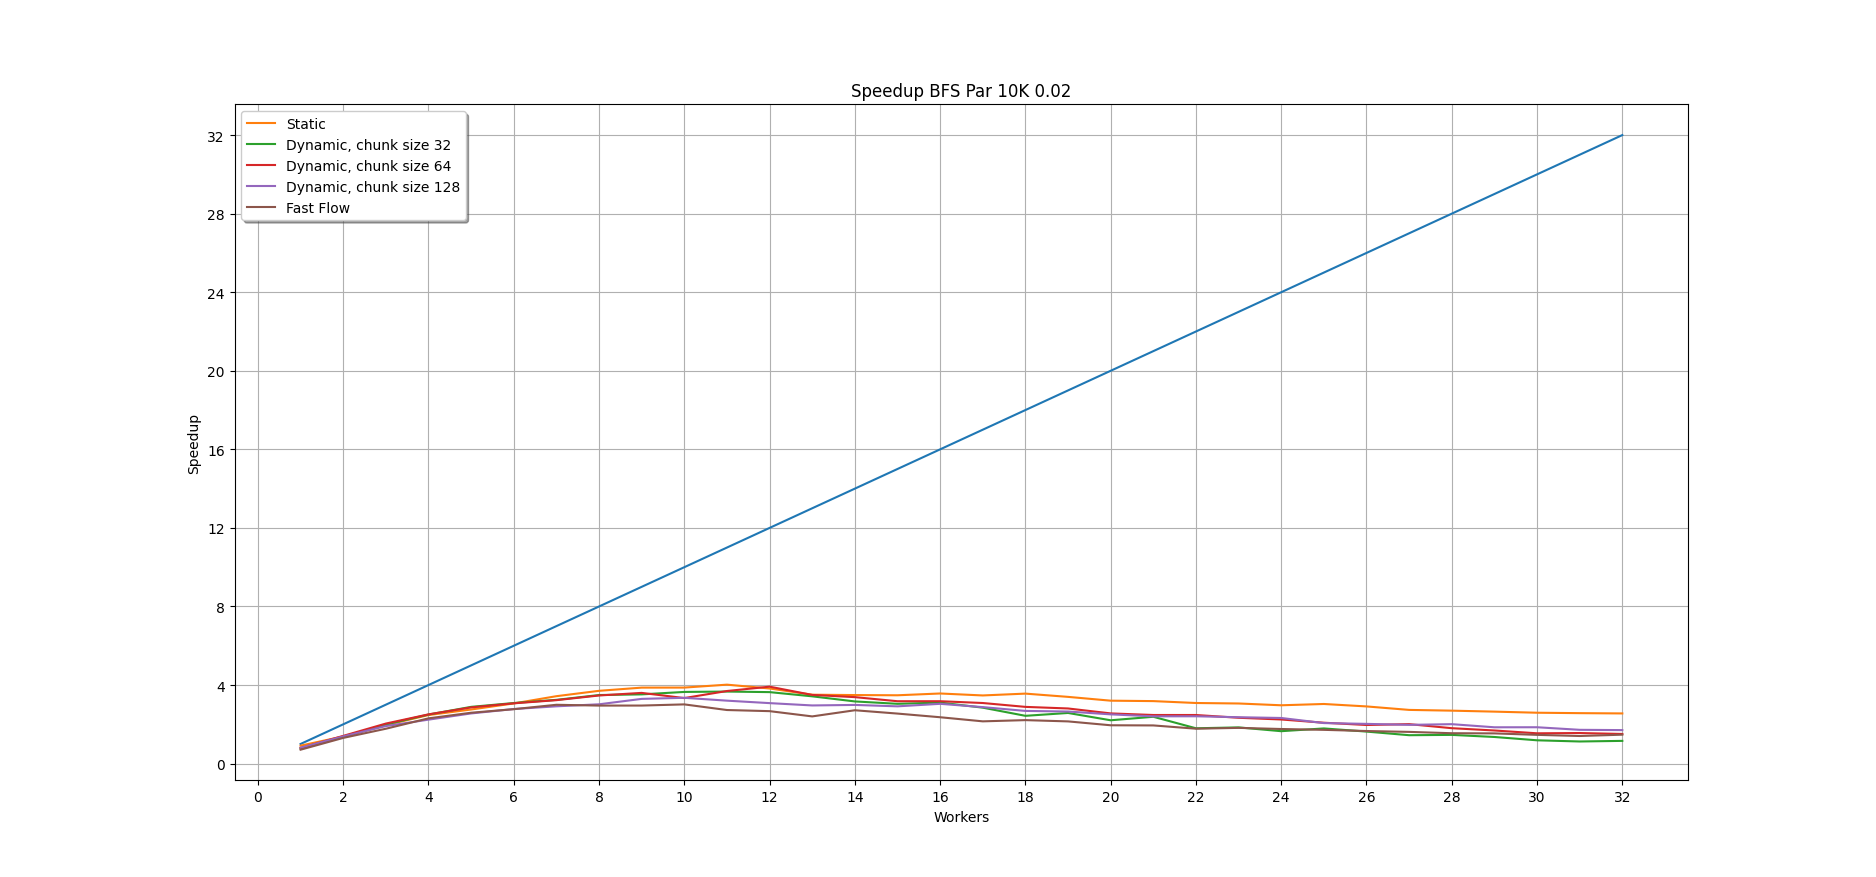
\includegraphics[width=0.75\textwidth]{Figures/plot_map_speedup_vs10K002.png}
    \caption{Speedup plot graph 0.02 density.}
    \label{fig:plot_speedup_10k_002}
\end{figure}
\FloatBarrier
Growing density to $0.5$, and so the frontier size, the static version starts to suffer of load balancing problems mainly in with lower $nw$. Indeed, static approaches, the speedup growth is limited by the large size of the chunks that give the possibility to the first workers to visit most of the graph nodes creating a bottleneck. Meanwhile, dividing the frontier in smaller chunks provides the possibility to handle efficiently the free workers. In fact, the dynamic verison performance are better, in particular for the version with chunk with $32$ nodes.

\begin{figure}[htb!]
    \centering
    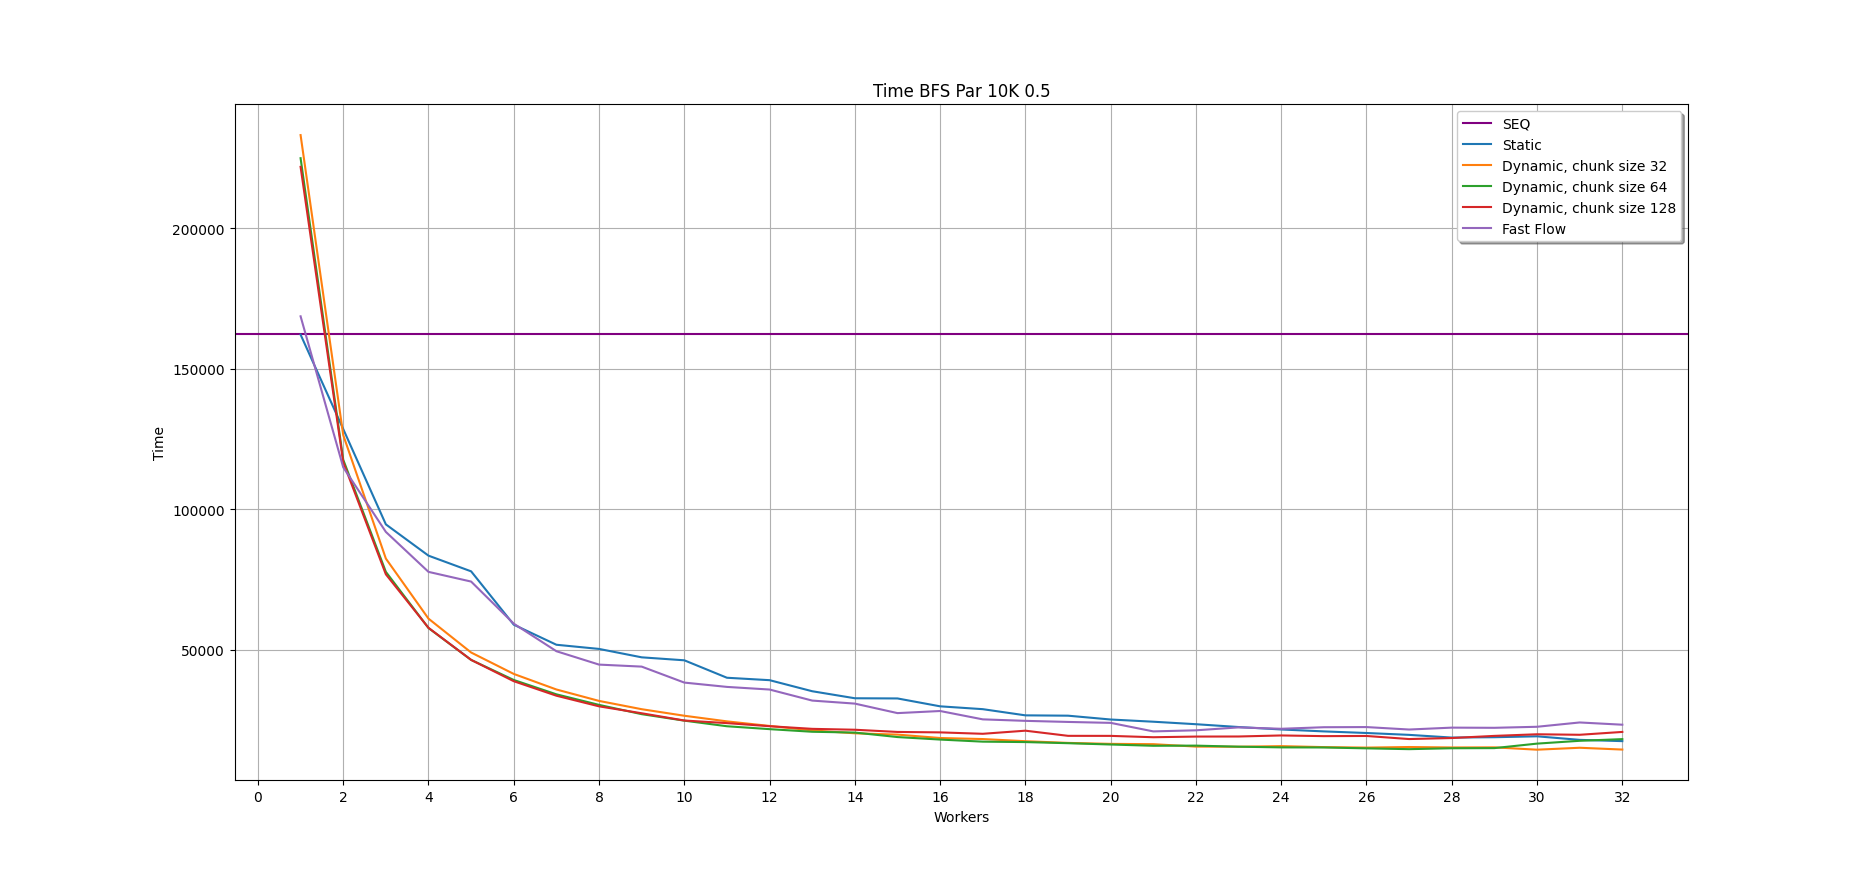
\includegraphics[width=0.75\textwidth]{Figures/plot_map_time_vs10K05.png}
    \caption{Time plot graph 0.5 density.}
    \label{fig:plot_time_10k_05}
\end{figure}
\FloatBarrier

\begin{figure}[htb!]
    \centering
    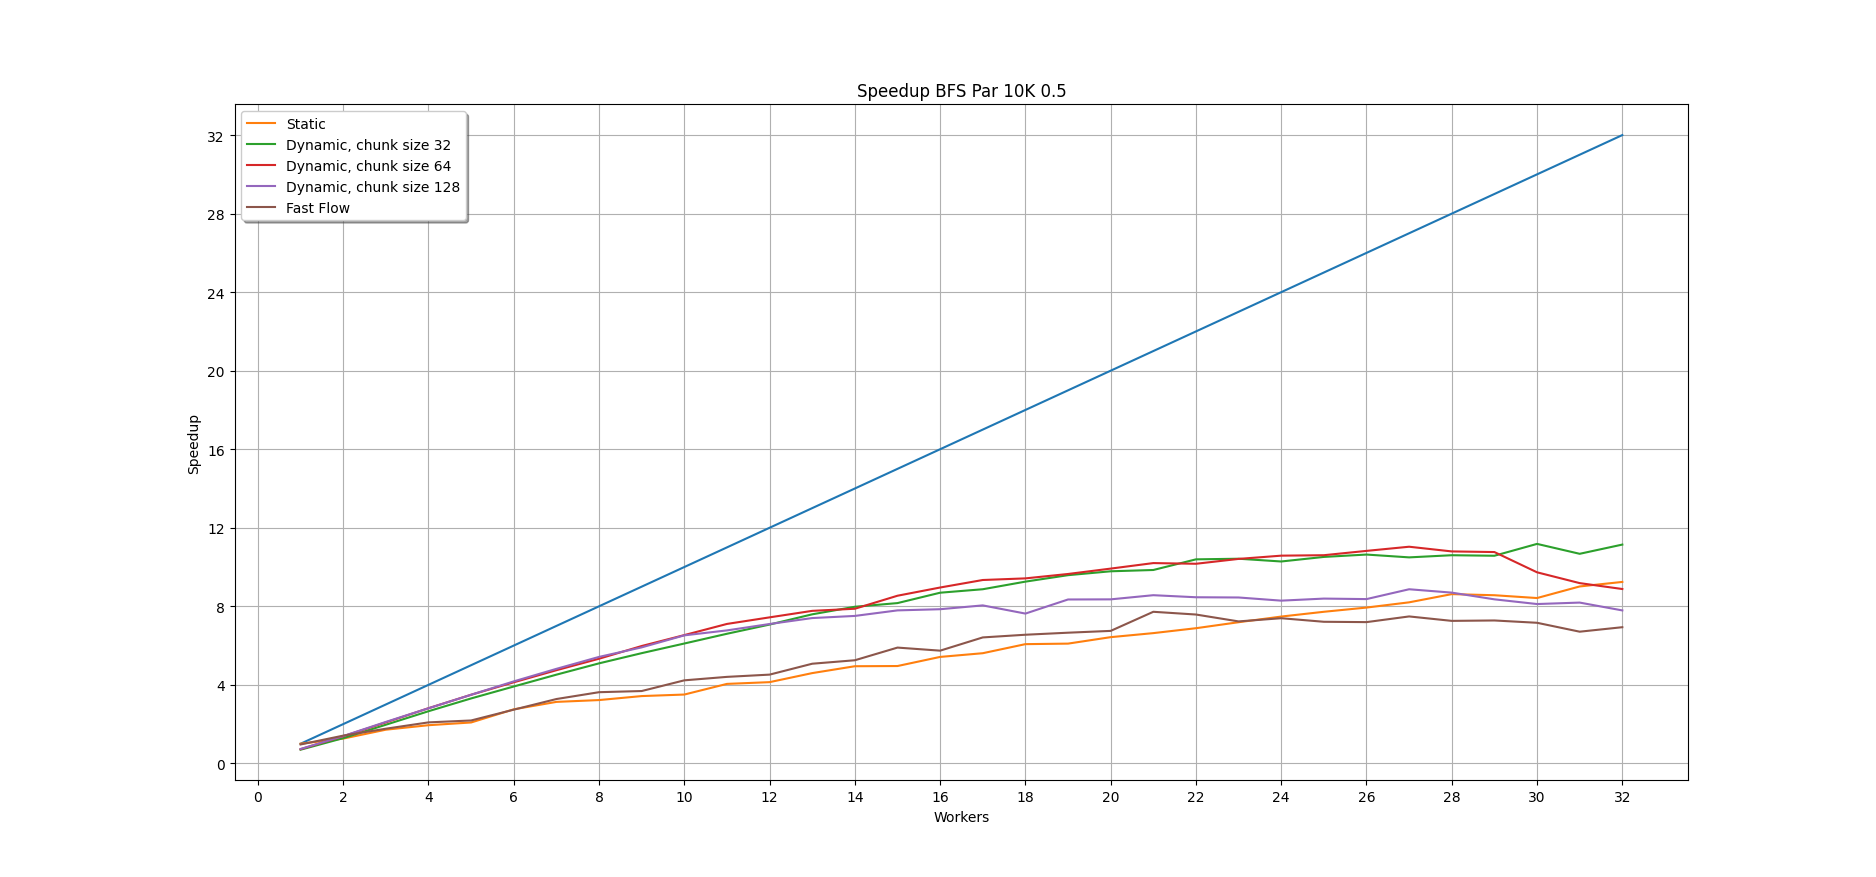
\includegraphics[width=0.75\textwidth]{Figures/plot_map_speedup_vs10K05.png}
    \caption{Speedup plot graph 0.5 density.}
    \label{fig:plot_speedup_10k_05}
\end{figure}
\FloatBarrier

The analysis of the last graph is almost the same and also in this case the Fast Flow version maintains a speedup margin about one point less than the version with static scheduling. This could be due to the task management by fast flow and for runs with many threads the need to re-execute $nw$ times the $svc$ method of the emitter with related checks. Also, for each new level of the graph the tasks are not reused but new ones are created, for very large frontiers this is a considerable overhead.

\begin{figure}[htb!]
    \centering
    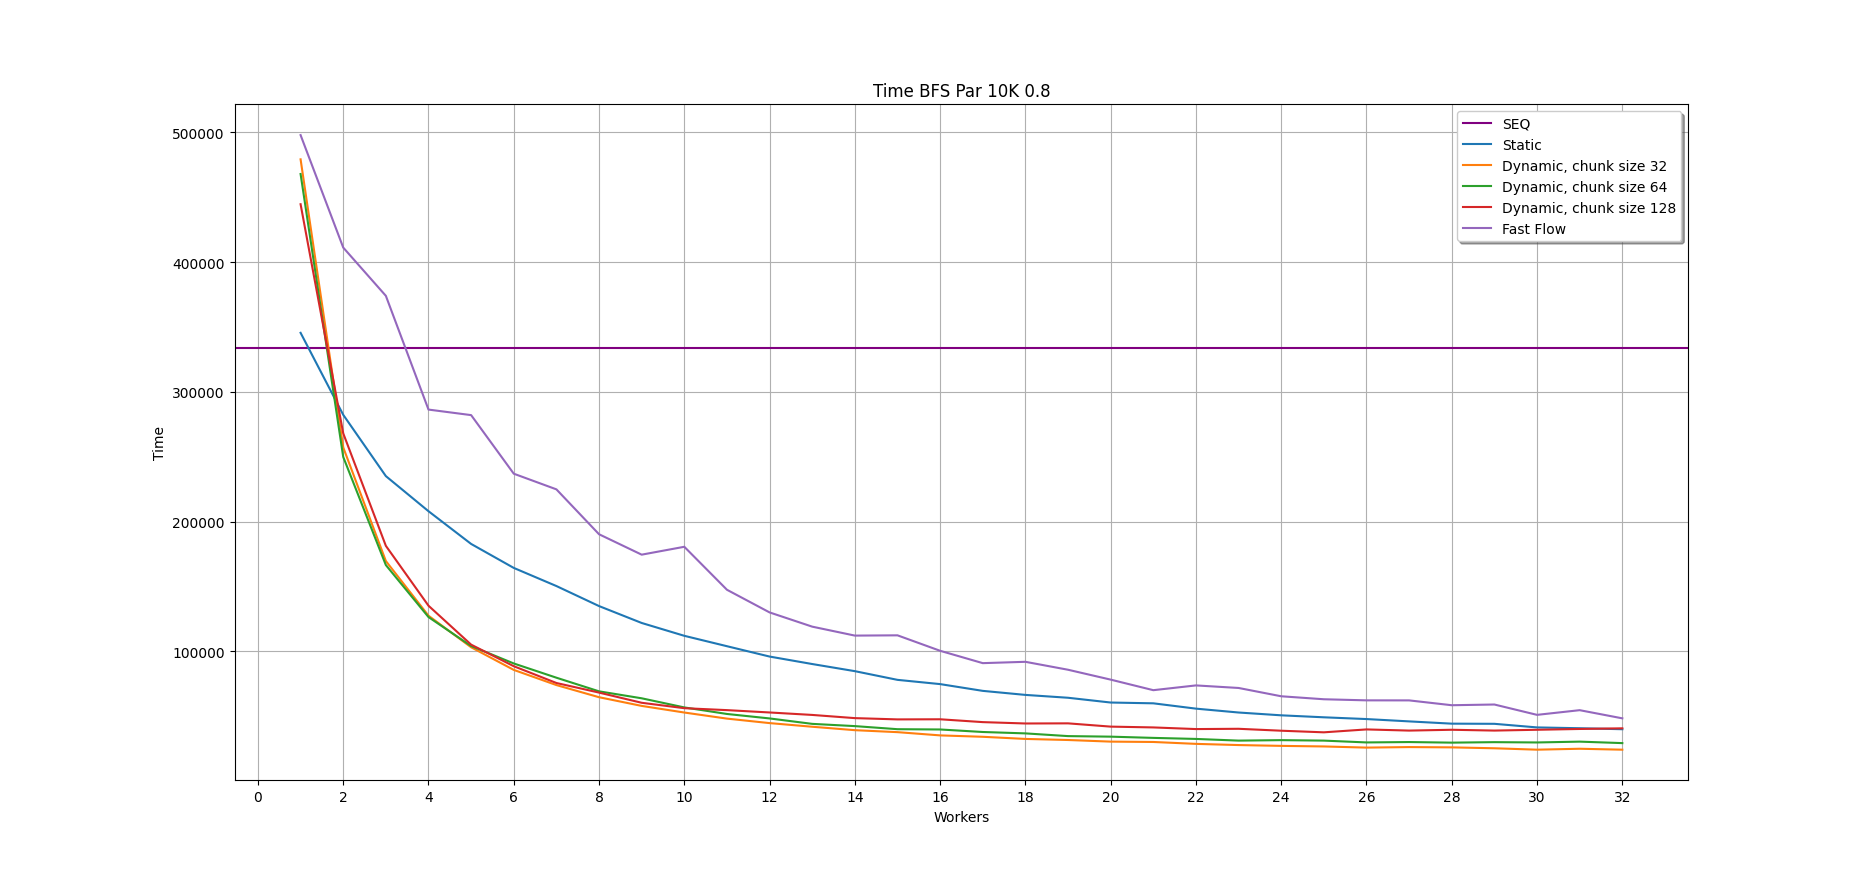
\includegraphics[width=0.75\textwidth]{Figures/plot_map_time_vs10K08.png}
    \caption{Time plot graph 0.8 density.}
    \label{fig:plot_time_10k_08}
\end{figure}
\FloatBarrier

\begin{figure}[htb!]
    \centering
    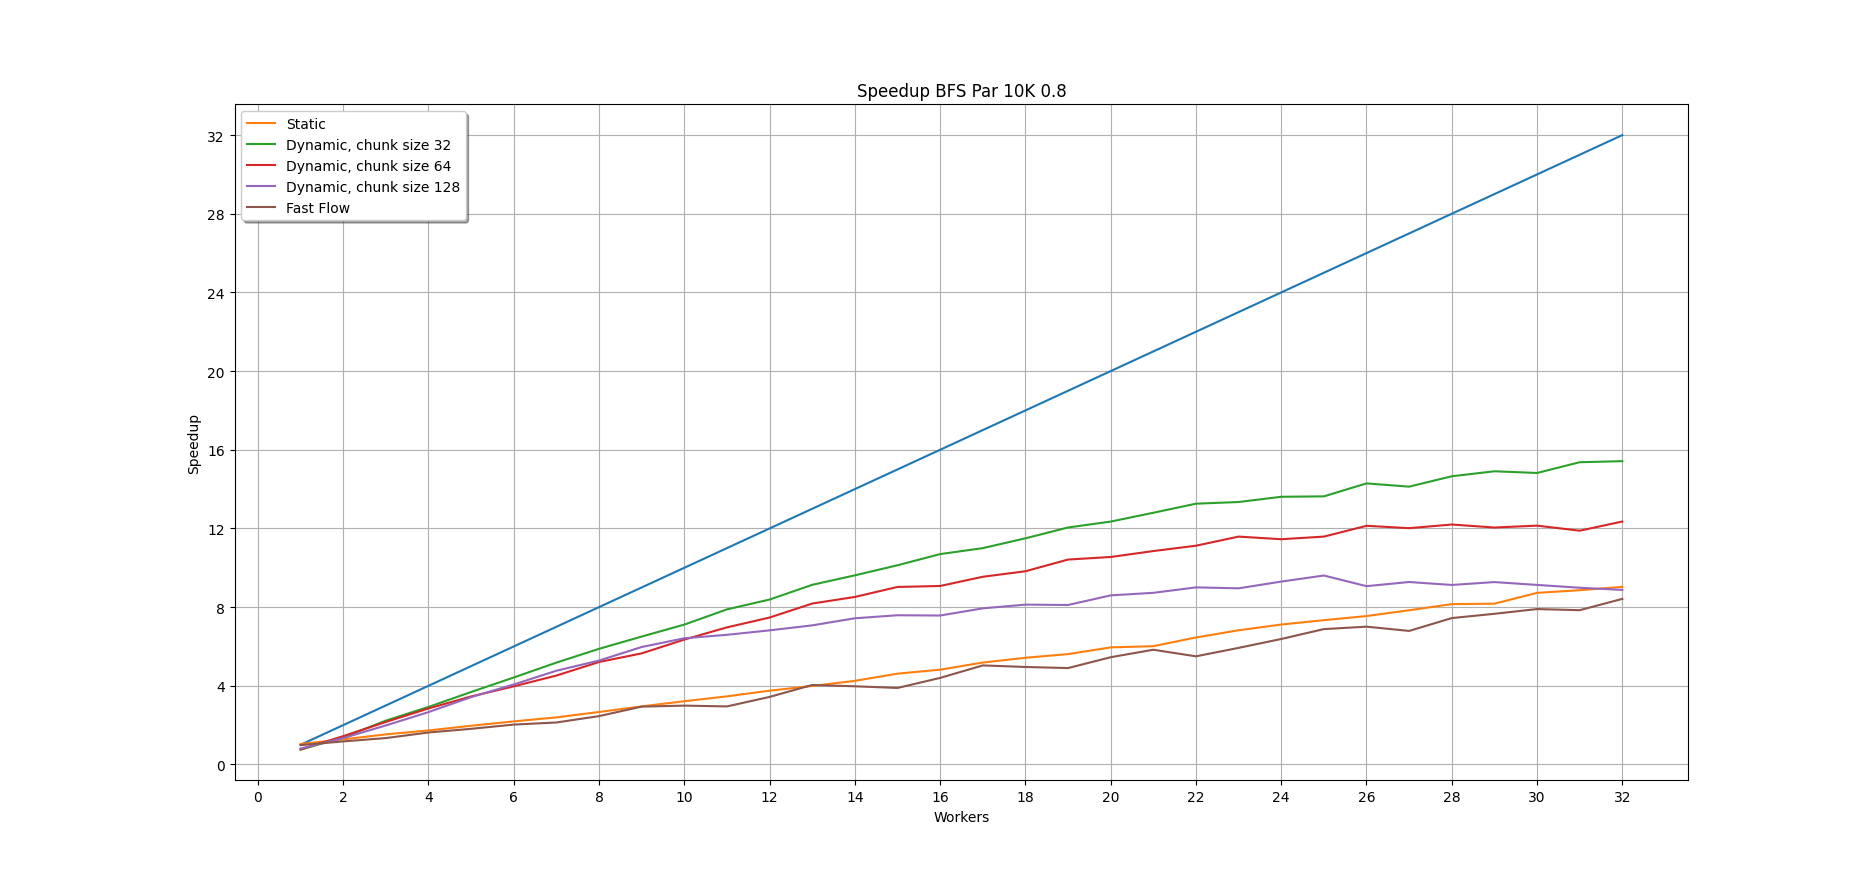
\includegraphics[width=0.75\textwidth]{Figures/plot_map_speedup_vs10K08.png}
    \caption{Speedup plot graph 0.8 density.}
    \label{fig:plot_speedup_10k_08}
\end{figure}
\FloatBarrier

In the following tables you can see the speedup trend from a numerical point of view for all versions.
\begin{table}[htb!]
\centering
\begin{tabular}{|c|c|c|c|}
\hline
Workers & 10K 0.02D & 10K 0.5D & 10K 0.8D \\ \hline
1       & 0,913606  & 1,001233 & 1,040779 \\ \hline
2       & 1,383123  & 1,262705 & 1,273857 \\ \hline
4       & 2,471753  & 1,943502 & 1,729321 \\ \hline
8       & 3,705753  & 3,223546 & 2,667787 \\ \hline
16      & 3,569641  & 5,421432 & 4,819437 \\ \hline
32      & 2,554548  & 9,240867 & 9,029531 \\ \hline
\end{tabular}
\caption{Speedup static scheduling.}
\label{table:spup_static}
\end{table}
\FloatBarrier

\begin{table}[htb!]
\centering
\begin{tabular}{|c|c|c|c|}
\hline
Workers & 10K 0.02D & 10K 0.5D & 10K 0.8D \\ \hline
1       & 0,708265  & 0,703803 & 0,791419 \\ \hline
2       & 1,308471  & 0,961453 & 0,943141 \\ \hline
4       & 2,303997  & 1,328917 & 1,39952  \\ \hline
8       & 2,953739  & 2,382475 & 2,059774 \\ \hline
16      & 2,360451  & 3,646711 & 3,770874 \\ \hline
32      & 1,472611  & 5,801207 & 7,44725  \\ \hline
\end{tabular}
\caption{Speedup Fast Flow solution.}
\label{table:spup_ff}
\end{table}
\FloatBarrier

\begin{table}[htb!]
\centering
\begin{tabular}{|c|c|c|c|}
\hline
Workers & 10K 0.02D & 10K 0.5D & 10K 0.8D \\ \hline
1       & 0,778865  & 0,696421 & 0,750639 \\ \hline
2       & 1,357478  & 1,284081 & 1,378061 \\ \hline
4       & 2,497896  & 2,655661 & 2,922916 \\ \hline
8       & 3,490782  & 5,093752 & 5,879286 \\ \hline
16      & 3,107527  & 8,691875 & 10,69519 \\ \hline
32      & 1,156913  & 11,14306 & 15,42083 \\ \hline
\end{tabular}
\caption{Speedup dynamic scheduling solution with chunk size of 32 nodes.}
\label{table:spup_dy}
\end{table}
\FloatBarrier